\documentclass[hyperref=colorlinks]{beamer}
\mode<presentation>
\usetheme{iclpt}
\setbeamertemplate{navigation symbols}{}
\setbeamertemplate{headline}{
\begin{beamercolorbox}[leftskip=.2cm,rightskip=.2cm,topskip=.2cm,ht=1.1cm,dp=0.1cm,wd=\textwidth]{institute in head/foot}
  
\includegraphics[height=1cm]{icl.pdf}
  \hfill
  
\includegraphics[height=1cm]{../Pics/CMS-Color.pdf}
\end{beamercolorbox}
}
\setbeamertemplate{footline}{
\begin{beamercolorbox}[ht=.55cm,dp=0.4cm,wd=\textwidth,leftskip=.3cm]{author in head/foot}%
  \begin{minipage}[c]{5cm}%
    \usebeamerfont{author in head/foot}
    \insertshortauthor 
    \insertshorttitle
    \end{minipage}\hfill%
  \insertframenumber{} / \pageref{lastframe}
  \hfill
  \begin{minipage}{6cm}
    \hfill
  \end{minipage}
\end{beamercolorbox}%
}

\usepackage{color}
\usepackage{tabularx,colortbl}
\usepackage{graphicx}
\usepackage{pdfpages}
\usepackage{feynmp}
\DeclareGraphicsRule{*}{mps}{*}{}

\title{\vspace{-0.2cm} VBF Higgs to Invisible - Update}
\subtitle{HIG-14-038, AN-14-243\vspace{-0.7cm}}
\author[P. Dunne]{\underline{P. Dunne}} % A.M. Magnan and A. Nikitenko Joao Pela with \\ R. Aggleton, J. Brooke: Bristol \\ C.Asawangtrakuldee, Q.Li: Peking \\ P. Srimanobhas: Chulalongkorn \\ S. Kumar, K. Mazumdar: Mumbai}
\titlegraphic{
  \vspace{-0.7cm}
  %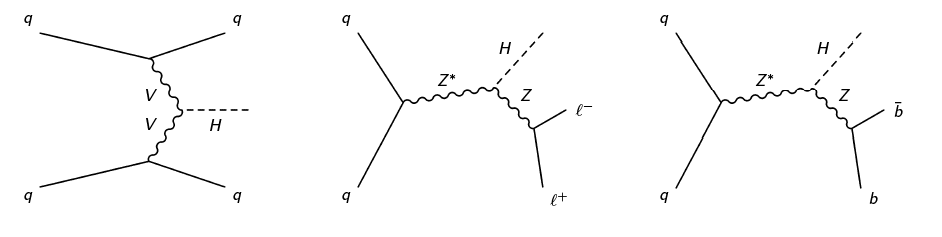
\includegraphics[width=\textwidth]{TalkPics/invcomb021213/feyndiags}
  %% \begin{fmfgraph*}(100,70)
  %%         \fmfleft{i1,i2}
  %%         \fmfright{o1,o2,o3}
  %%         \fmf{fermion}{i1,v1,o1}
  %%         \fmf{fermion}{i2,v2,o3}
  %%         \fmf{phantom,tension=4/5}{v1,v2}
  %%         \fmffreeze
  %%         \fmf{photon,label=$W,,Z$}{v1,v3}
  %%         \fmf{photon,label=$W,,Z$}{v2,v3}
  %%         \fmf{dashes}{v3,o2}
  %%         \fmflabel{$q$}{i1}
  %%         \fmflabel{$q$}{i2}
  %%         \fmflabel{$q$}{o1}
  %%         \fmflabel{$q$}{o3}
  %%         \fmflabel{$H$}{o2}
  %%       \end{fmfgraph*}
}
\date{}
\begin{document}
\begin{fmffile}{higgsexoupdatefeyndiags}

%TITLE PAGE
\section{Title}
\begin{frame}
  \titlepage
  
\end{frame}

\begin{frame}
  \frametitle{Overview}
  \begin{block}{}
    \scriptsize
    \begin{itemize}
    \item Preapproval conditions:
    \item[-] Clarify documentation
    \item[-] Investigate tau veto
    \item[-] Get data cards approved by comb group
    \item[-] Closure tests
    \item Documentation clarified:
    \item[-] Lepton scale factors referred to in section 4.2
    \item[-] Top scale factor use clarified in W background section
    \item Other points addressed in below slides
    \end{itemize}
  \end{block}
\end{frame}

\begin{frame}
  \frametitle{Tau veto}
  \begin{block}{}
    \scriptsize
    \begin{itemize}
    \item Added tau veto to signal region
    \item Background estimate reduced by 5 events ($\sim 1\%$)
    \item No change in signal yield
    \item Gain much smaller than 8\% systematic on tau ID efficiency
    \item We propose not to add a tau veto
    \end{itemize}
  \end{block}
\end{frame}

\begin{frame}
  \frametitle{Datacard approval}
  \begin{block}{}
    \scriptsize
      \begin{itemize}
      \item Comb group suggested using gmN uncertainty for low stats Z control region
      \item Current dummy ``observation'' in datacards is just expected background
      \item On changing to gmN prefit expected limit goes from 0.38 to 0.42
      \item[-] postfit to dummy ``observed'' limit goes to 0.39
      \item Difference between postfit and prefit is odd as the ``observed'' and expected number of events is the same
      \item Artefact of poor behaviour of asymptotic for prefit gmN uncertainties
      \item Ran expected limit with full toys, result is 0.39
      \item Cards given green light by Nick
      \end{itemize}
    \end{block}
\end{frame}

\begin{frame}
  \frametitle{Closure Test Procedure}
  \begin{block}{}
    \scriptsize
    \begin{itemize}
    \item Want to validate background in a region close to the signal region
    \item[-] QCD or signal contamination prevent use of most areas
    \item Predict yield in other control regions using munu control region
    \item Three entries in plots on next few slides:
    \item[-] Raw MC: MC estimate in control region under study
    \item[-] Data: Observed yield in control region under study
    \item[-] Data-Driven: Raw MC multiplied by data/MC scale factor from munu region
    \item Data driven scale factor is calculated bin by bin
    \item Band in ratio plot is systematic error on Data-Driven/Data ratio
    \item[-] Indicative only as correlations present
    \end{itemize}
  \end{block}
  
\end{frame}

%OUTLINE
\begin{frame}
  \frametitle{enu closure}
  \begin{block}{}
    \centering
    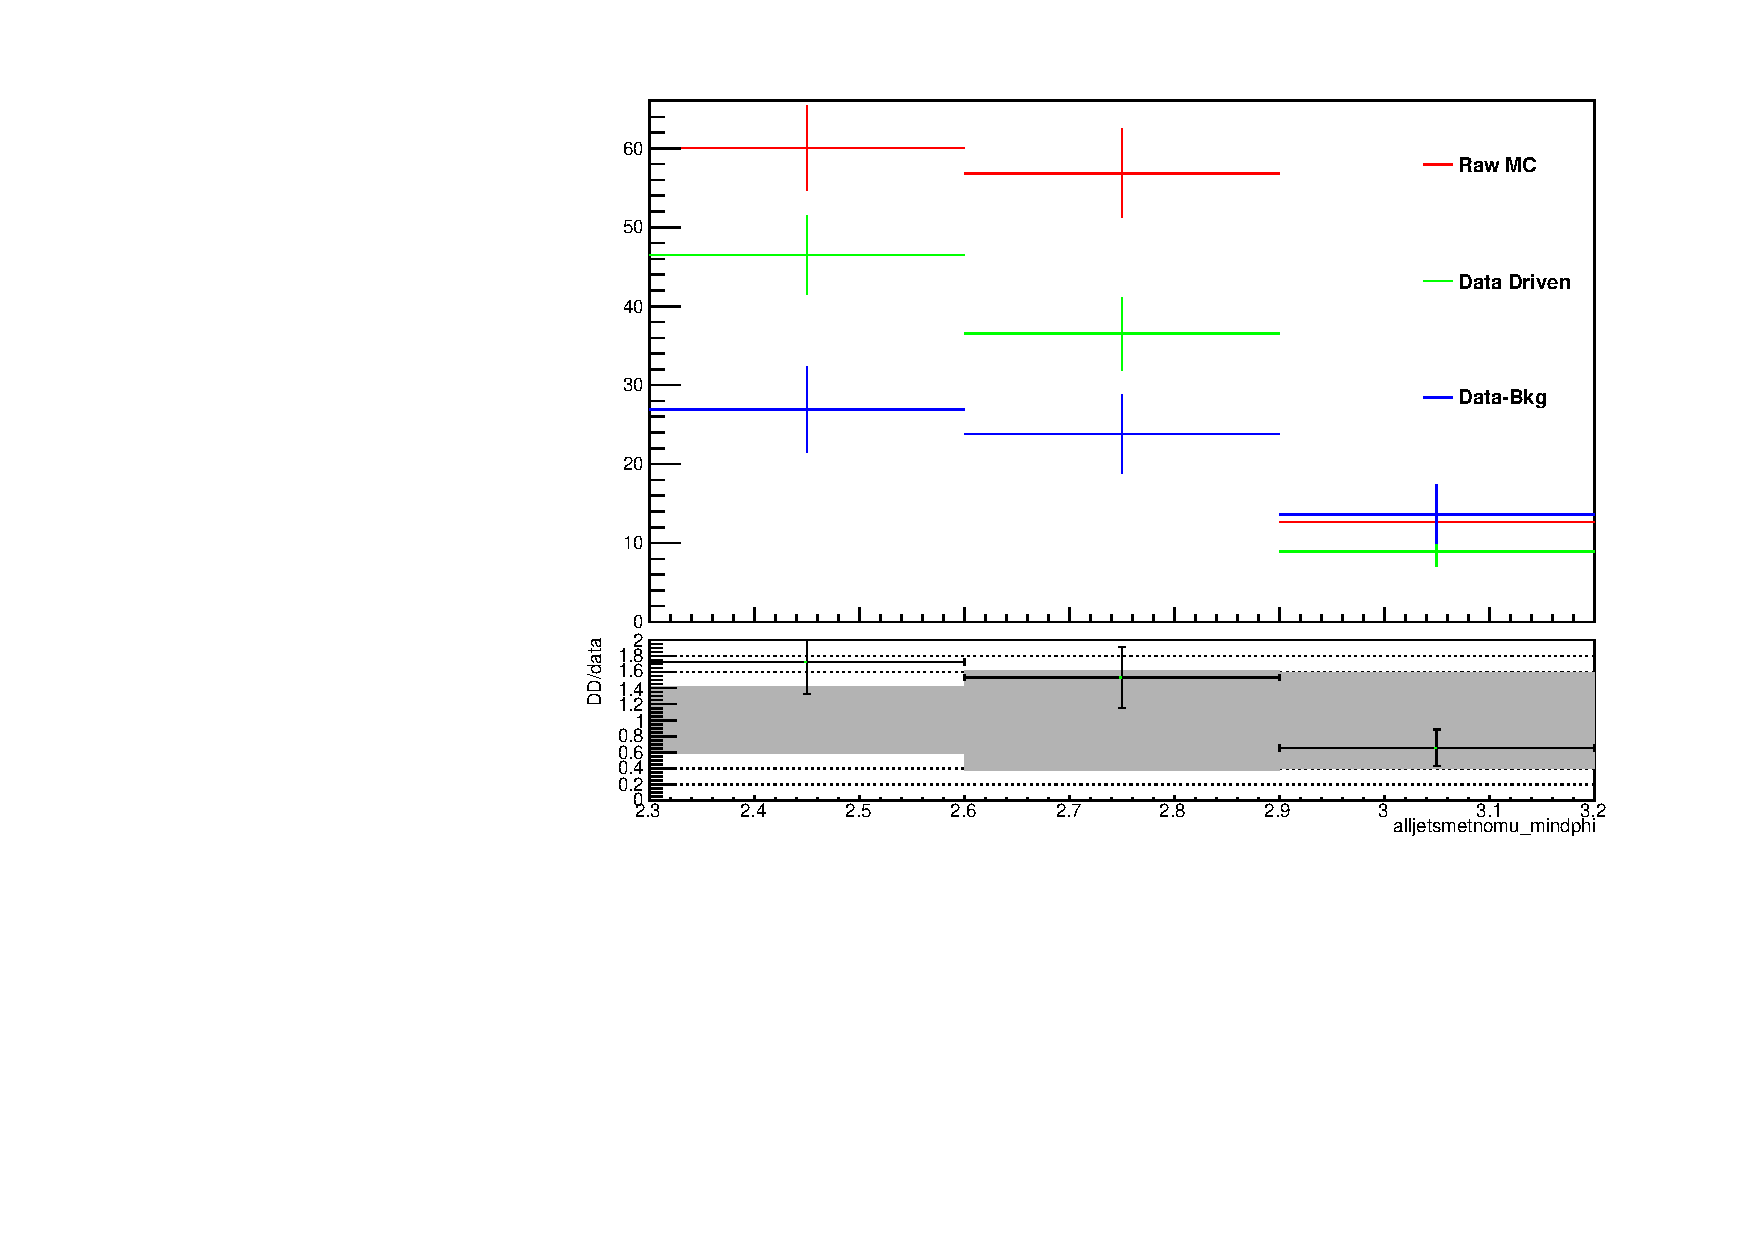
\includegraphics[width=.8\textwidth]{TalkPics/closuretests171214/closurealljetsmetnomu_mindphiWJets_enu.pdf}
  \end{block}
\end{frame}

\begin{frame}
  \frametitle{enu closure}
  \begin{block}{}
    \centering
    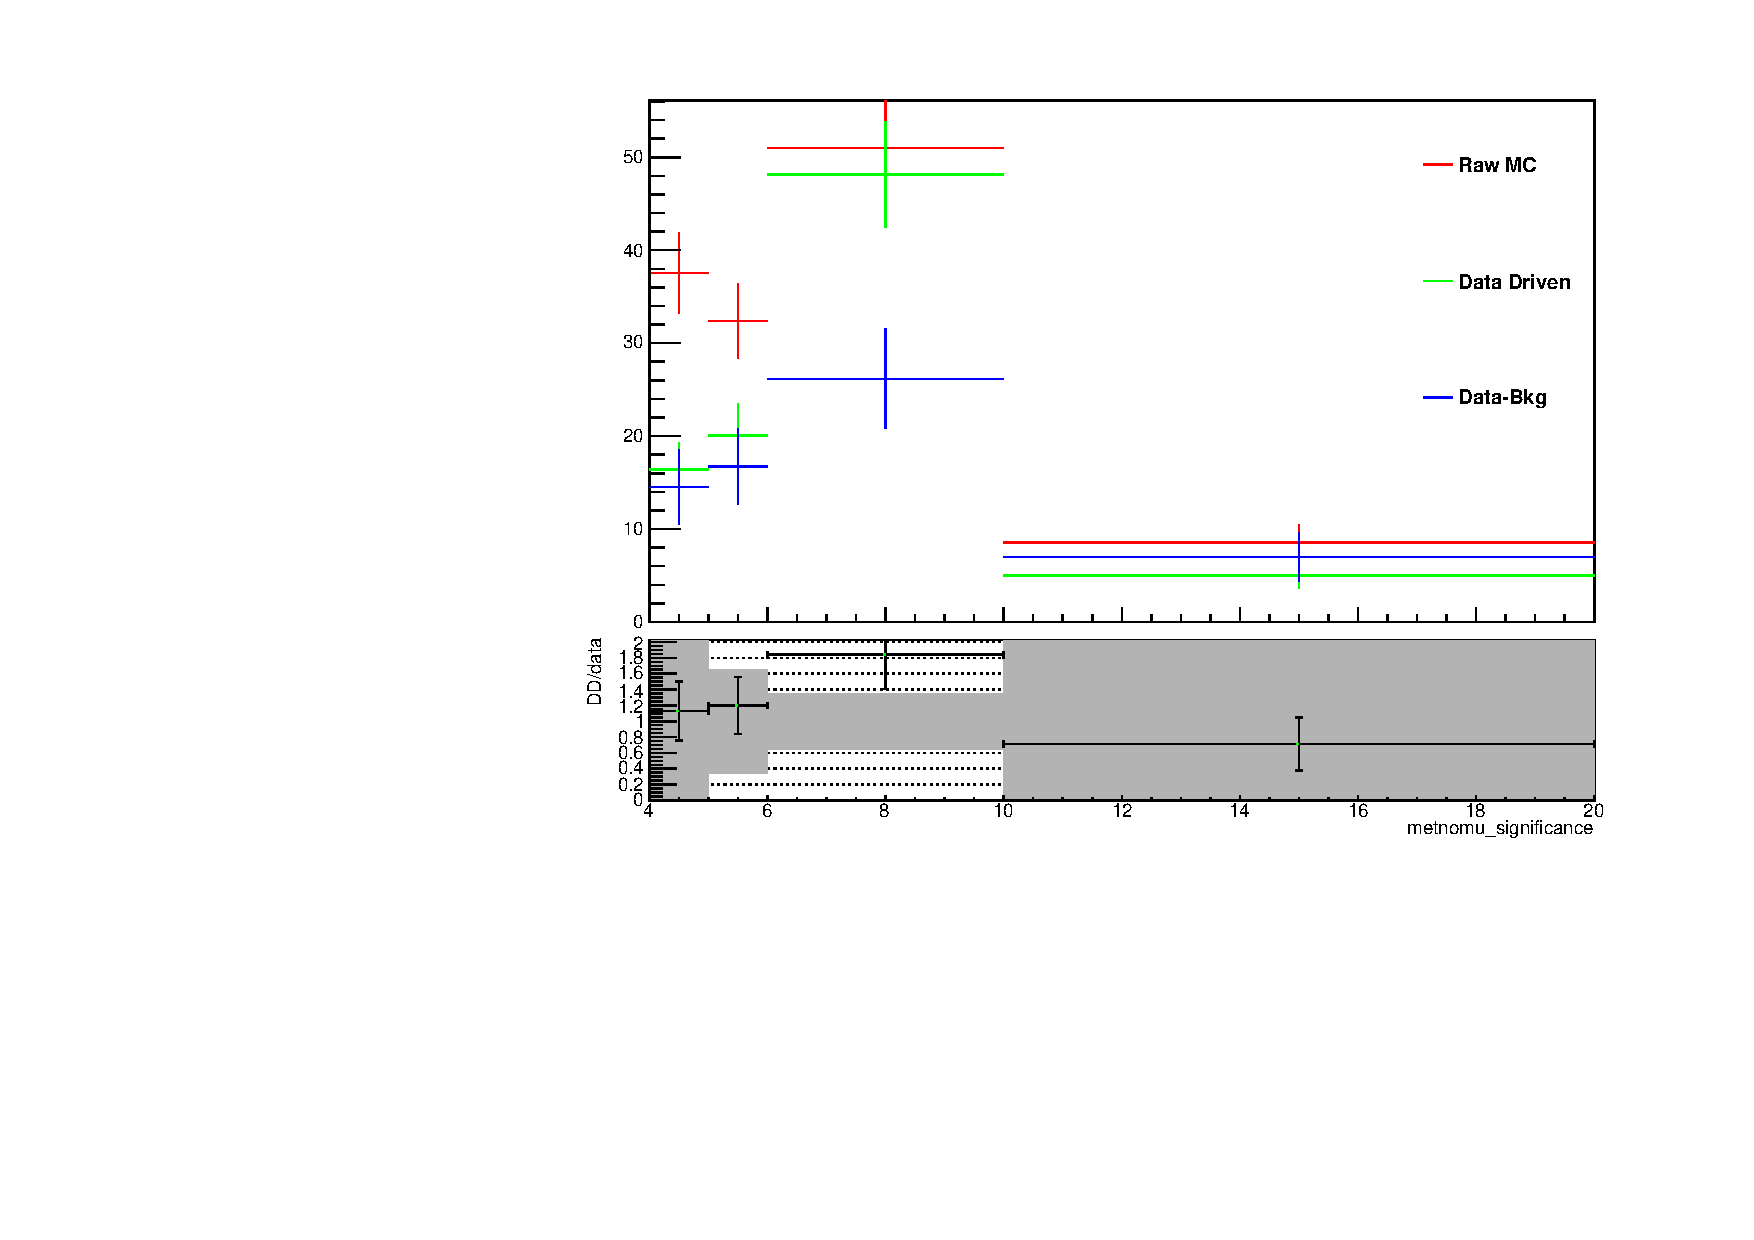
\includegraphics[width=.8\textwidth]{TalkPics/closuretests171214/closuremetnomu_significanceWJets_enu.pdf}
  \end{block}
\end{frame}

\begin{frame}
  \frametitle{enu closure}
  \begin{block}{}
    \centering
    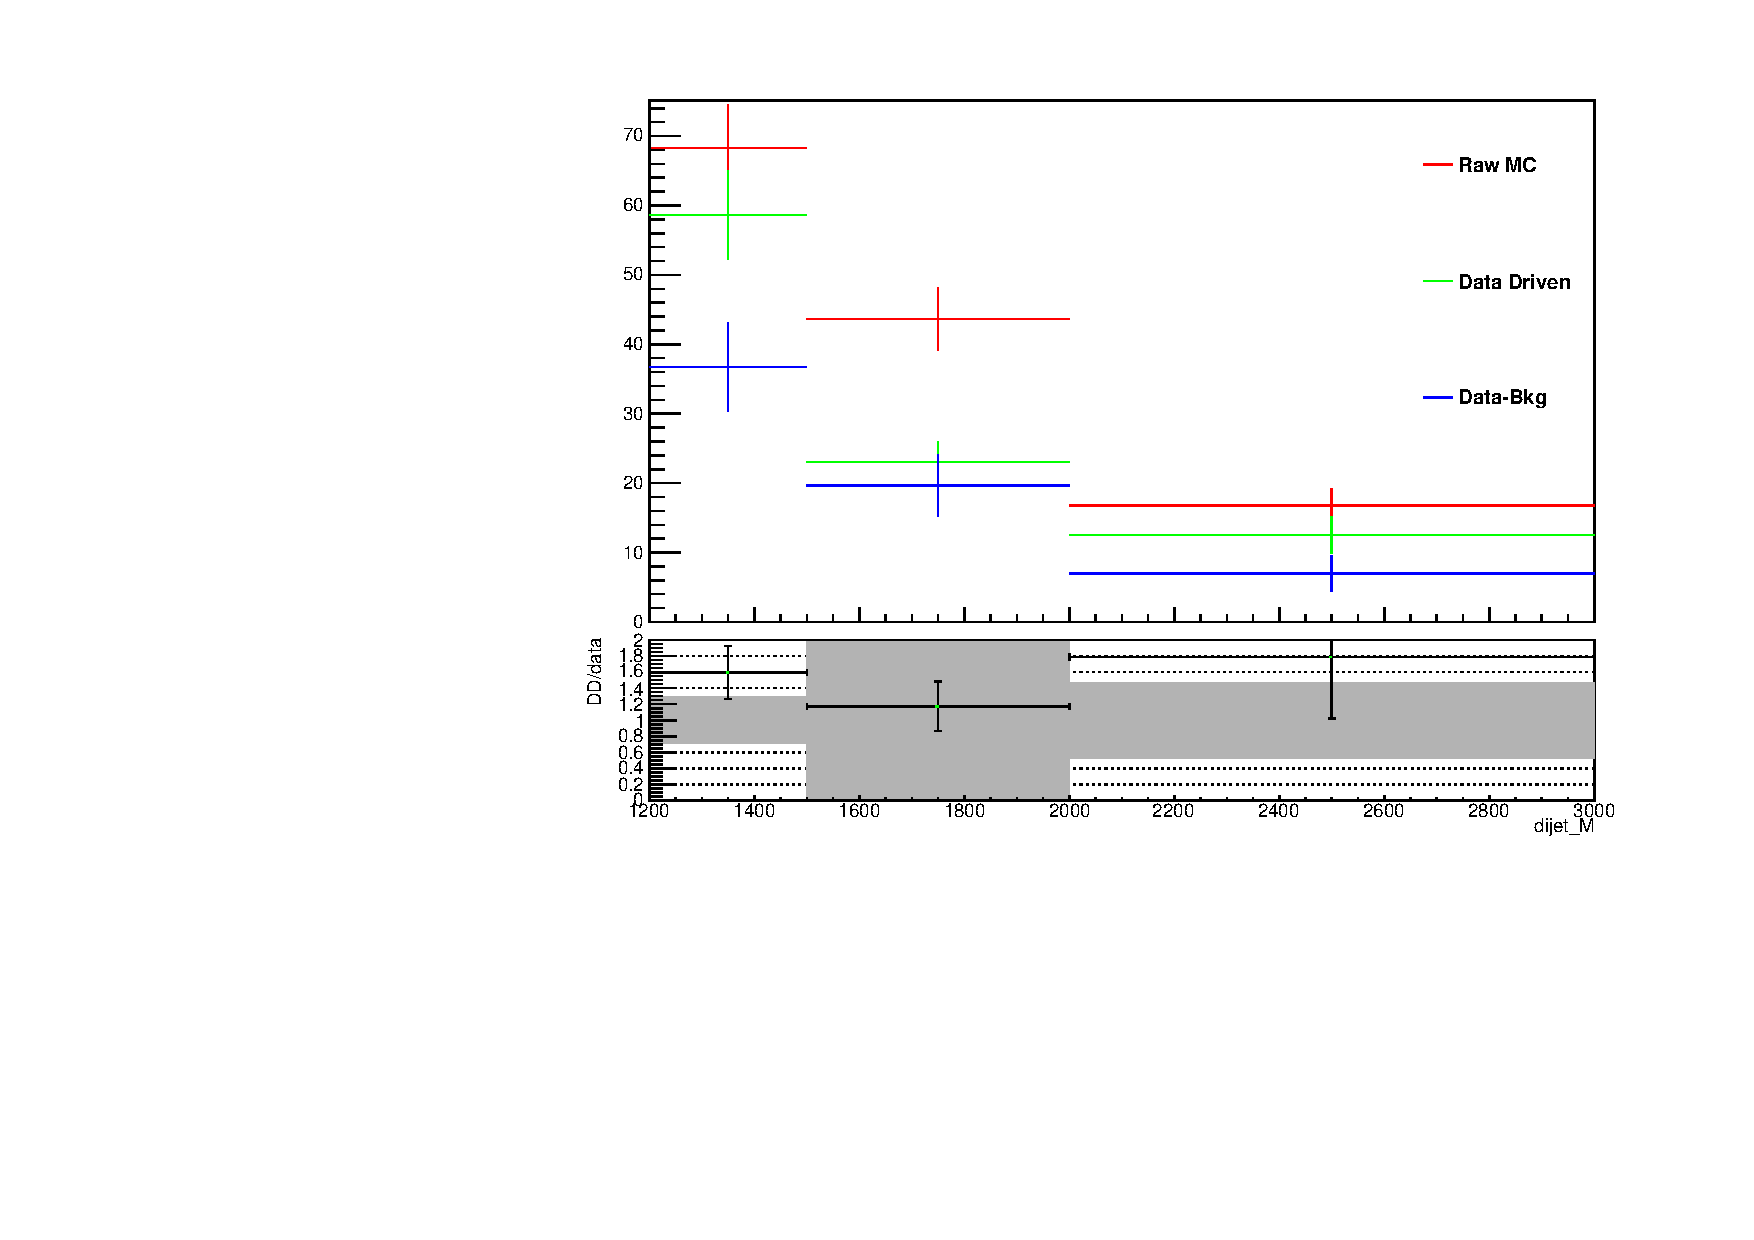
\includegraphics[width=.8\textwidth]{TalkPics/closuretests171214/closuredijet_MWJets_enu.pdf}
  \end{block}
\end{frame}

\begin{frame}
  \frametitle{enu closure}
  \begin{block}{}
    \centering
    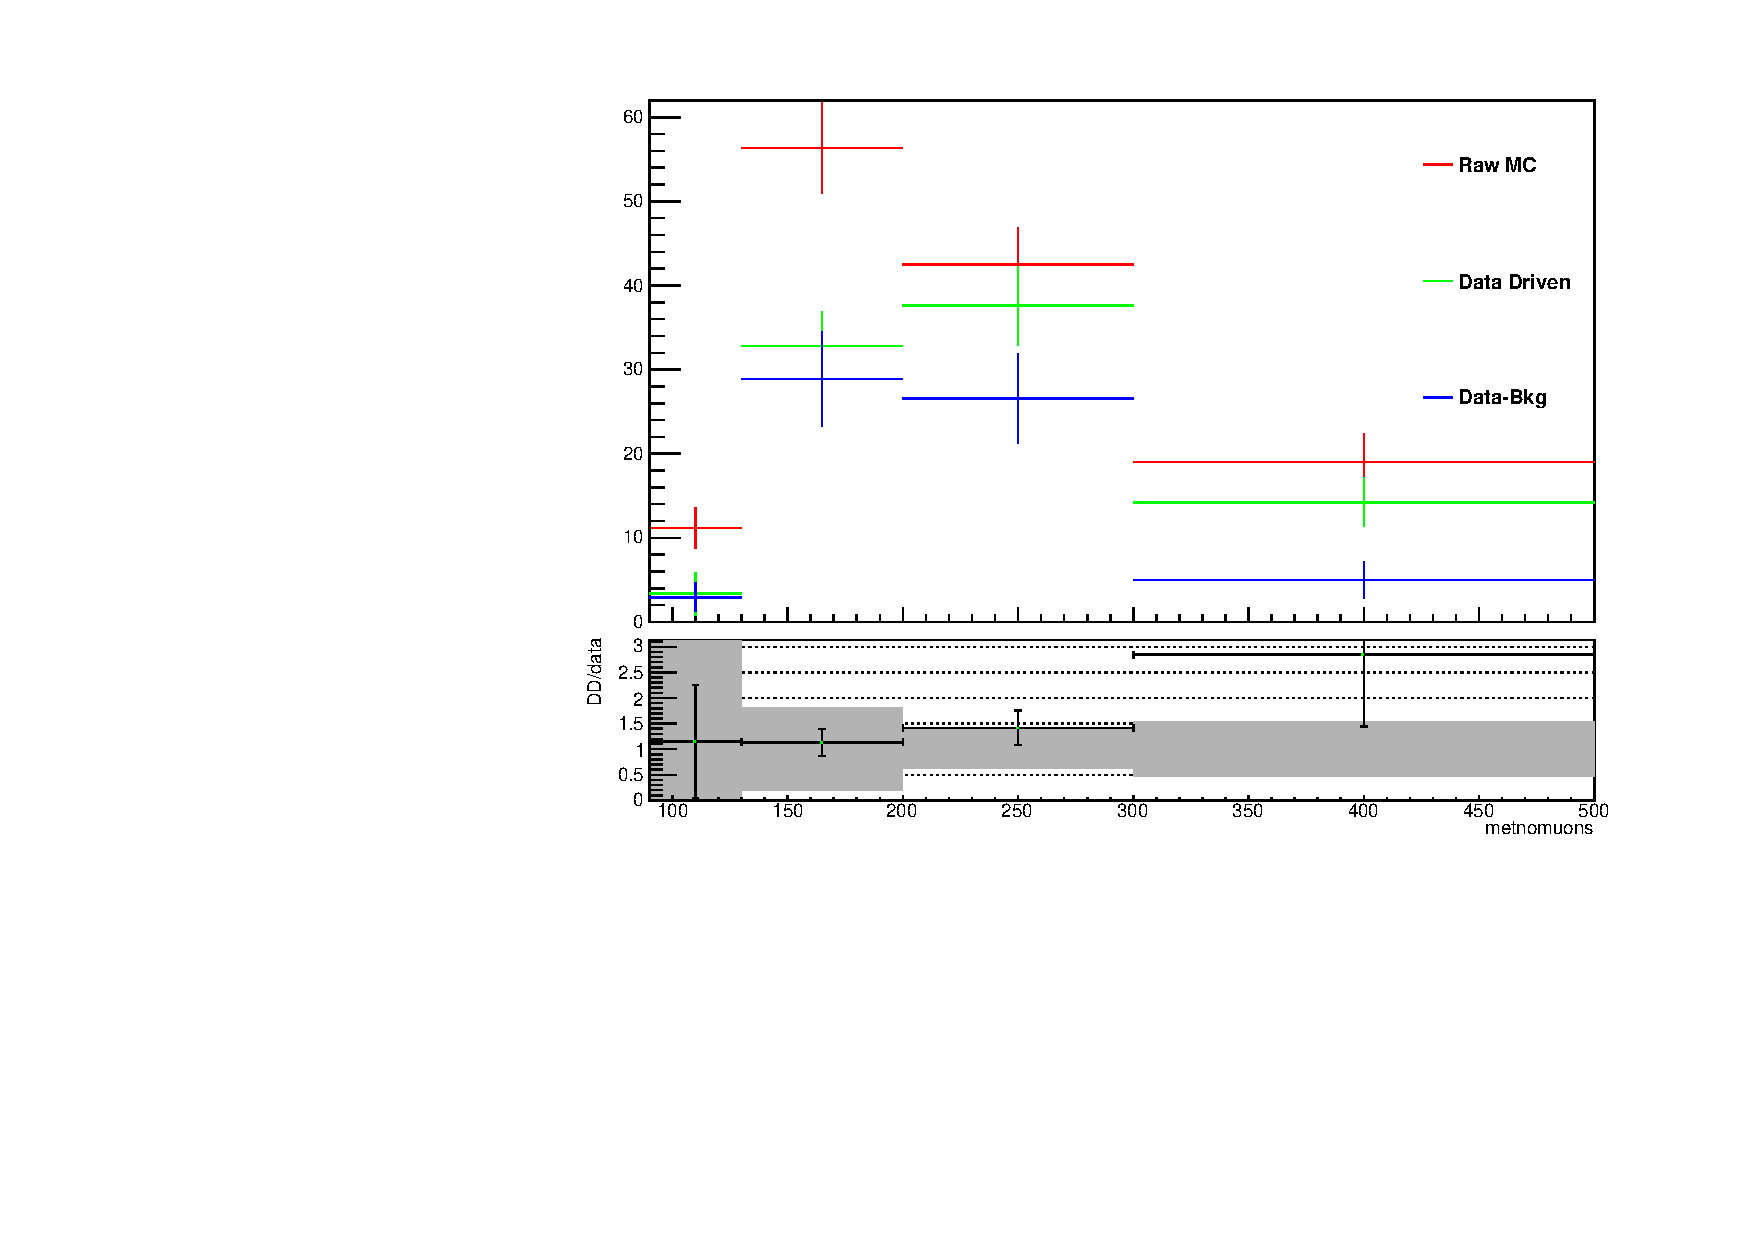
\includegraphics[width=.8\textwidth]{TalkPics/closuretests171214/closuremetnomuonsWJets_enu.pdf}
  \end{block}
\end{frame}

\begin{frame}
  \frametitle{taunu closure}
  \begin{block}{}
    \centering
    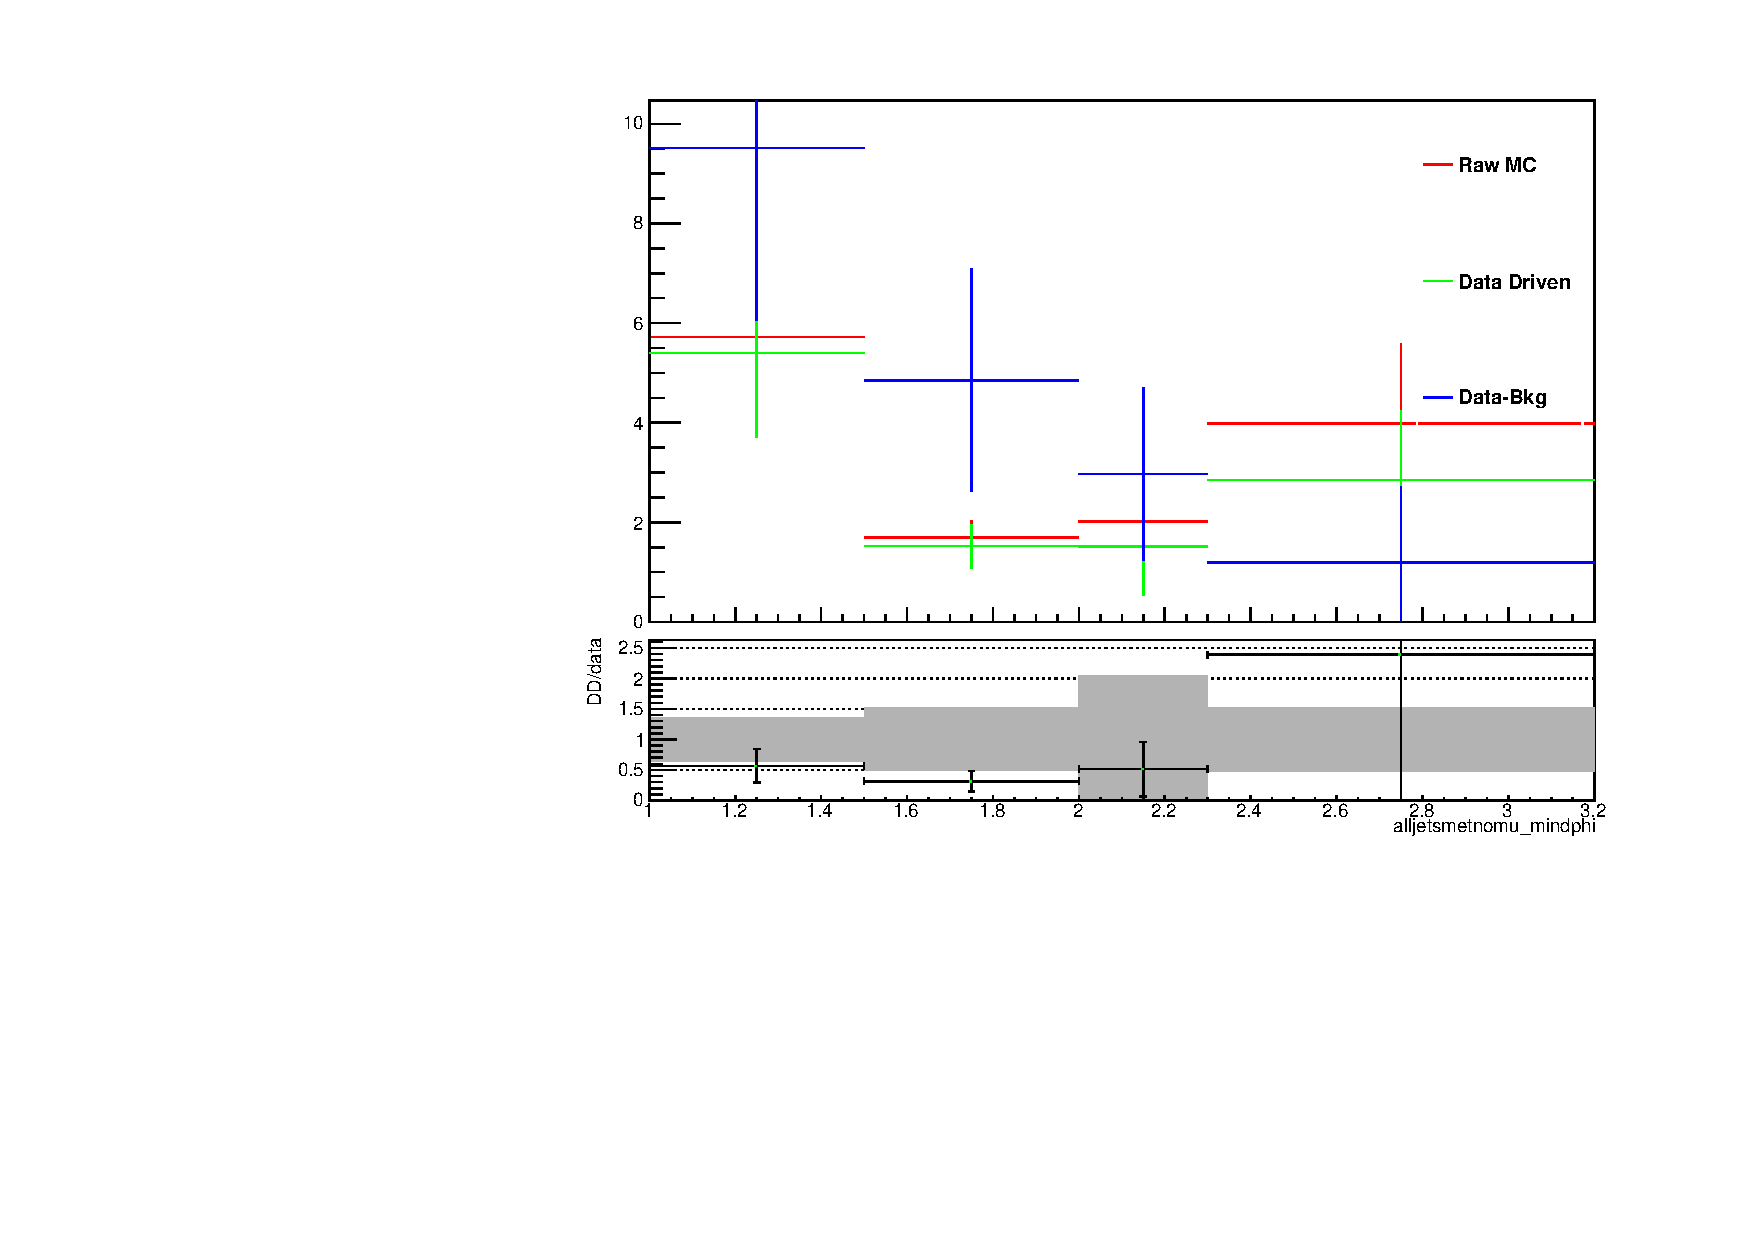
\includegraphics[width=.8\textwidth]{TalkPics/closuretests171214/closurealljetsmetnomu_mindphiWJets_taunu.pdf}
  \end{block}
\end{frame}

\begin{frame}
  \frametitle{taunu closure}
  \begin{block}{}
    \centering
    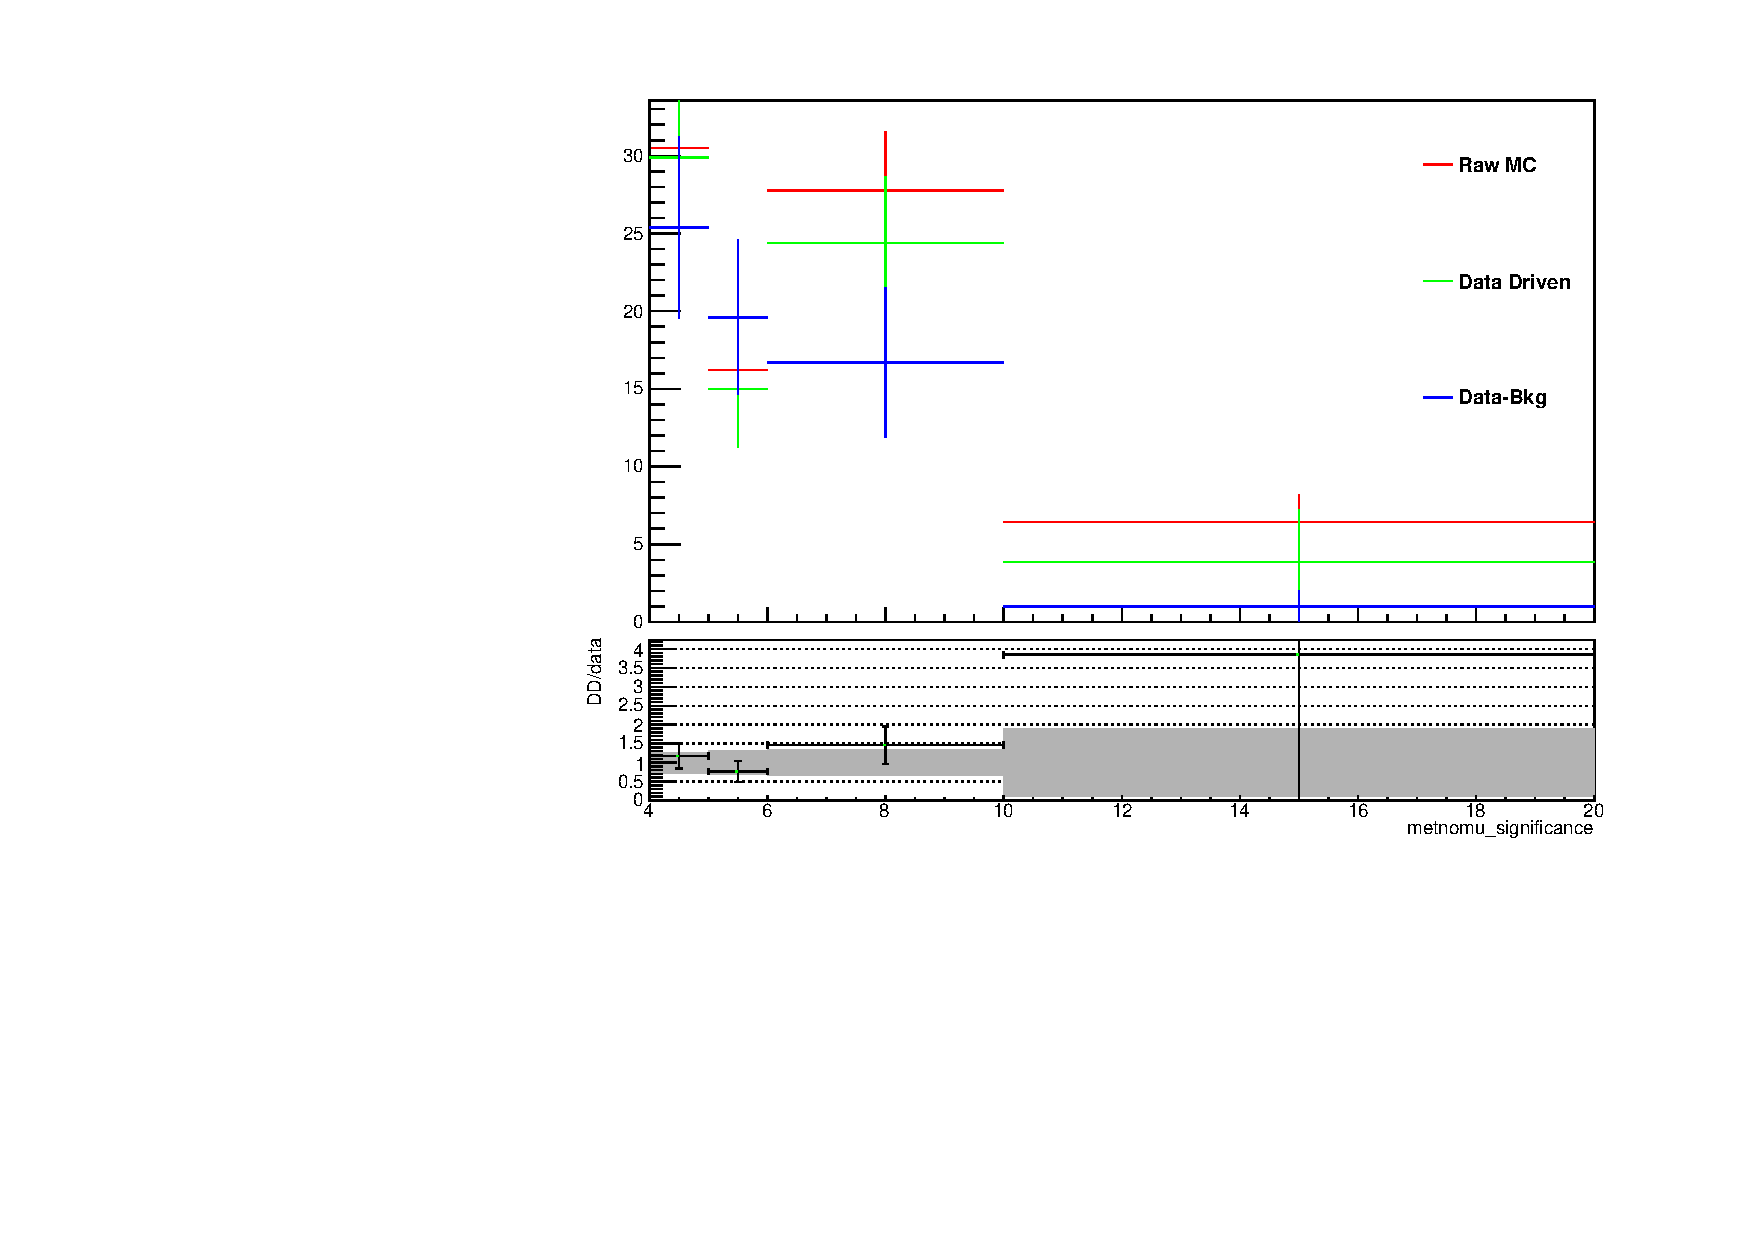
\includegraphics[width=.8\textwidth]{TalkPics/closuretests171214/closuremetnomu_significanceWJets_taunu.pdf}
  \end{block}
\end{frame}

\begin{frame}
  \frametitle{taunu closure}
  \begin{block}{}
    \centering
    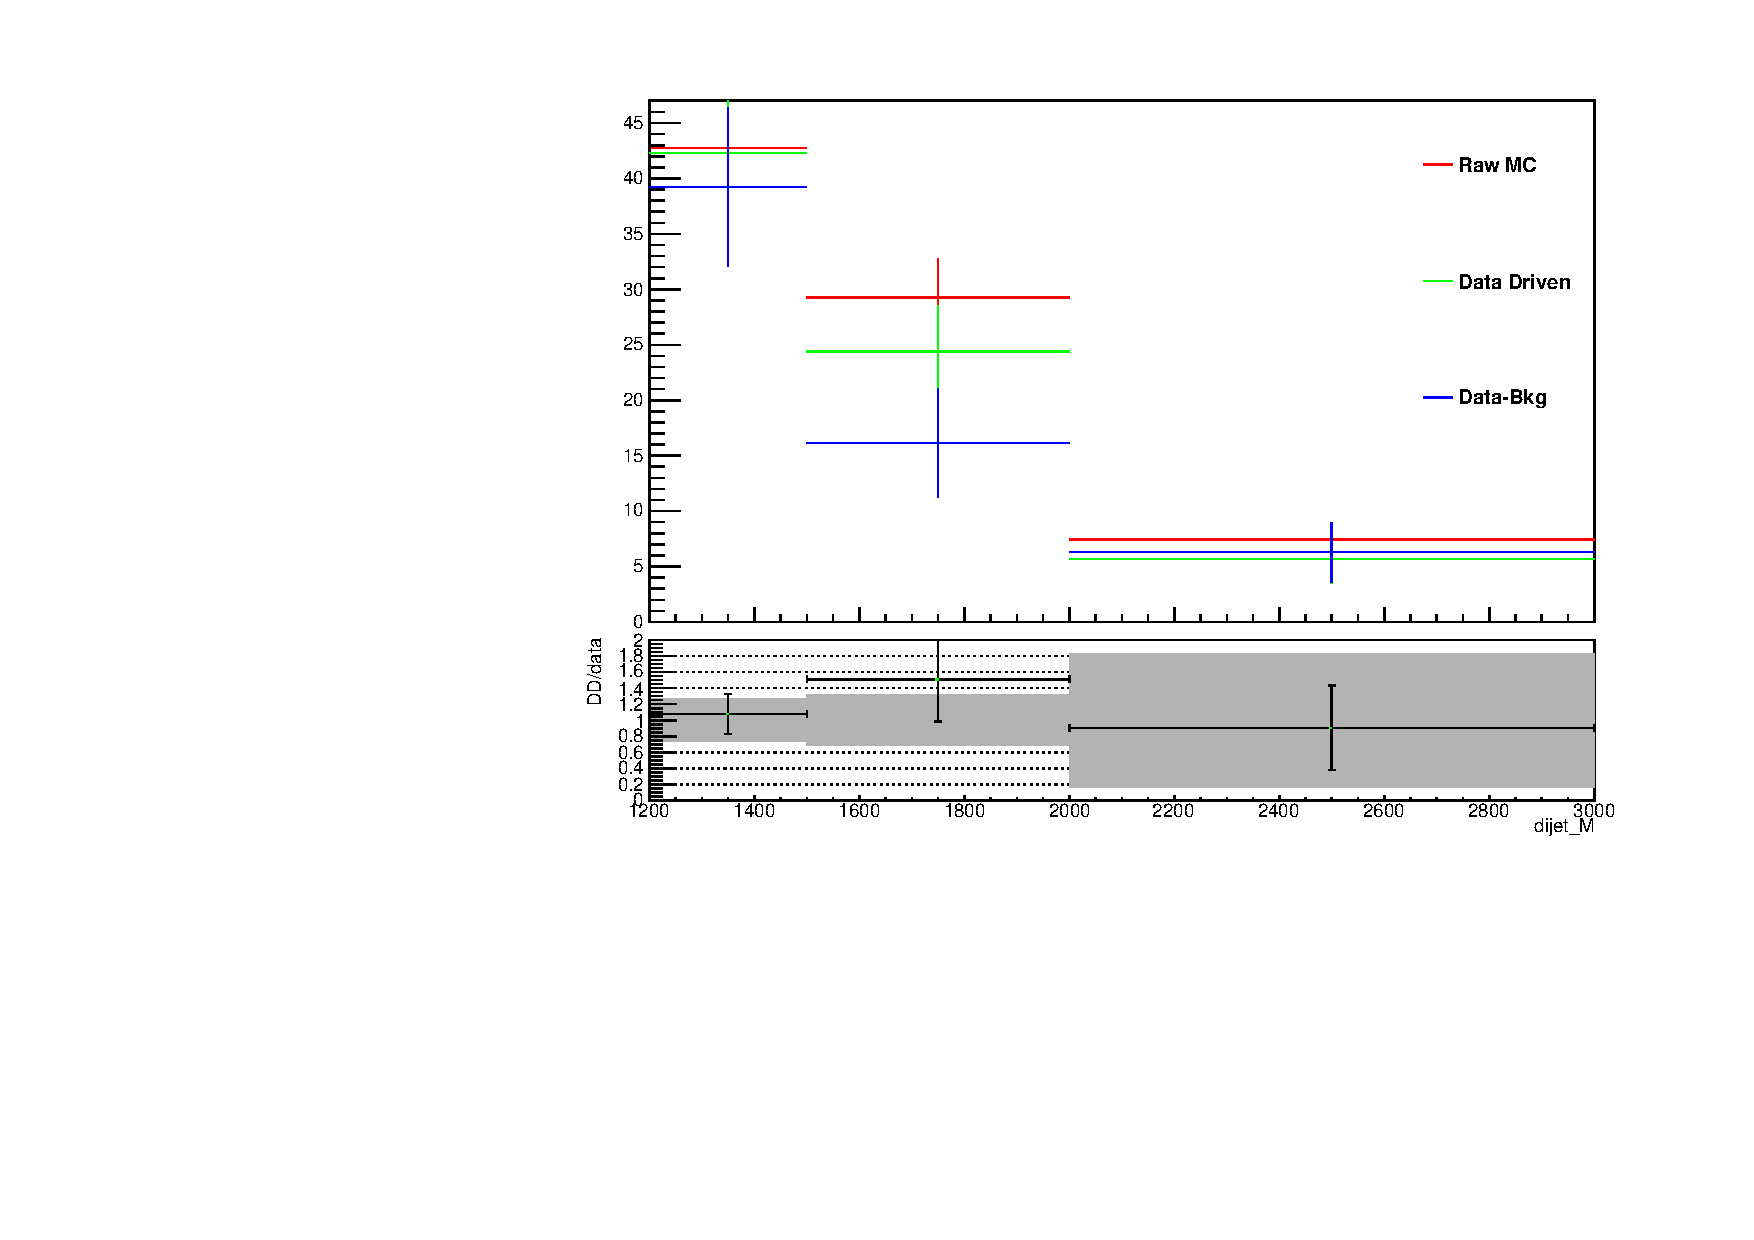
\includegraphics[width=.8\textwidth]{TalkPics/closuretests171214/closuredijet_MWJets_taunu.pdf}
  \end{block}
\end{frame}

\begin{frame}
  \frametitle{taunu closure}
  \begin{block}{}
    \centering
    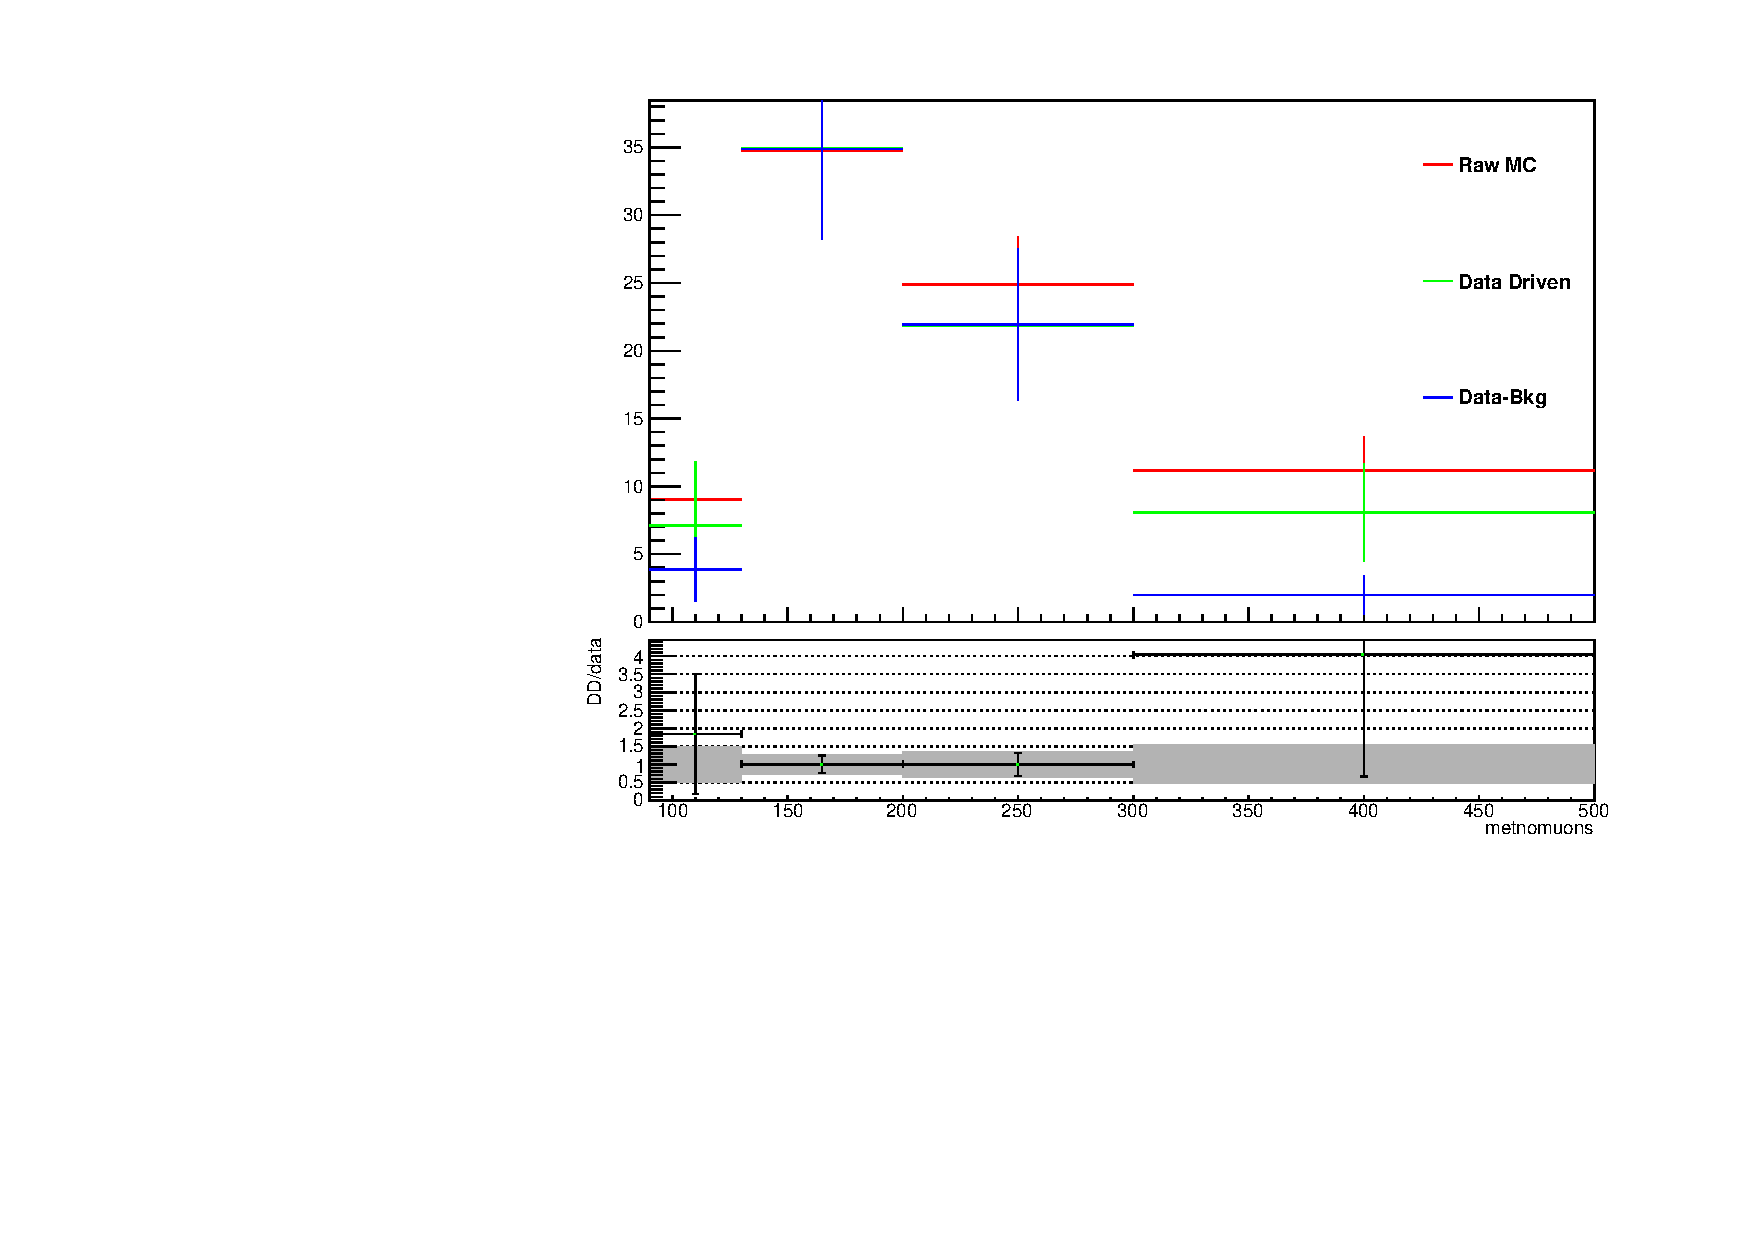
\includegraphics[width=.8\textwidth]{TalkPics/closuretests171214/closuremetnomuonsWJets_taunu.pdf}
  \end{block}
\end{frame}

\begin{frame}
  \frametitle{mumu closure}
  \begin{block}{}
    \centering
    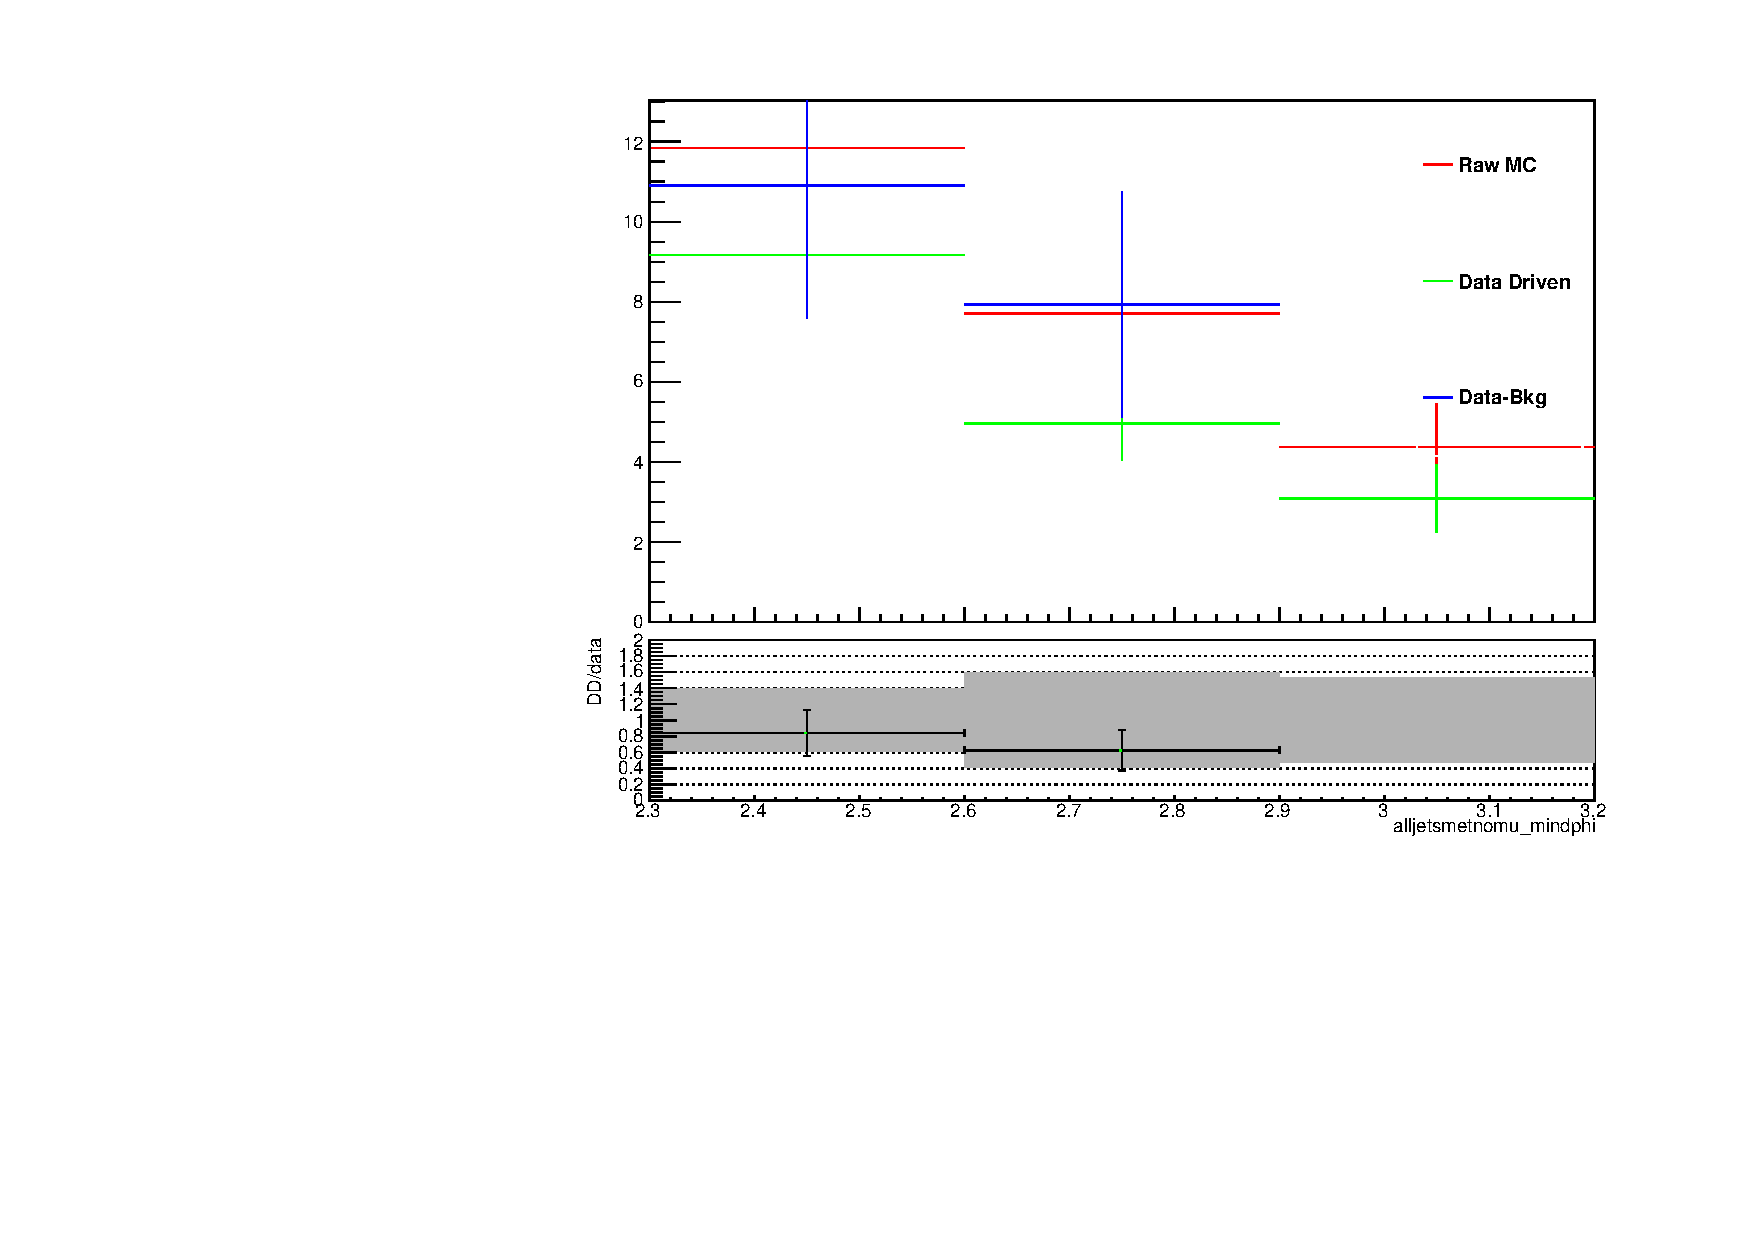
\includegraphics[width=.8\textwidth]{TalkPics/closuretests171214/closurealljetsmetnomu_mindphiZJets_ll_all.pdf}
  \end{block}
\end{frame}

\begin{frame}
  \frametitle{mumu closure}
  \begin{block}{}
    \centering
    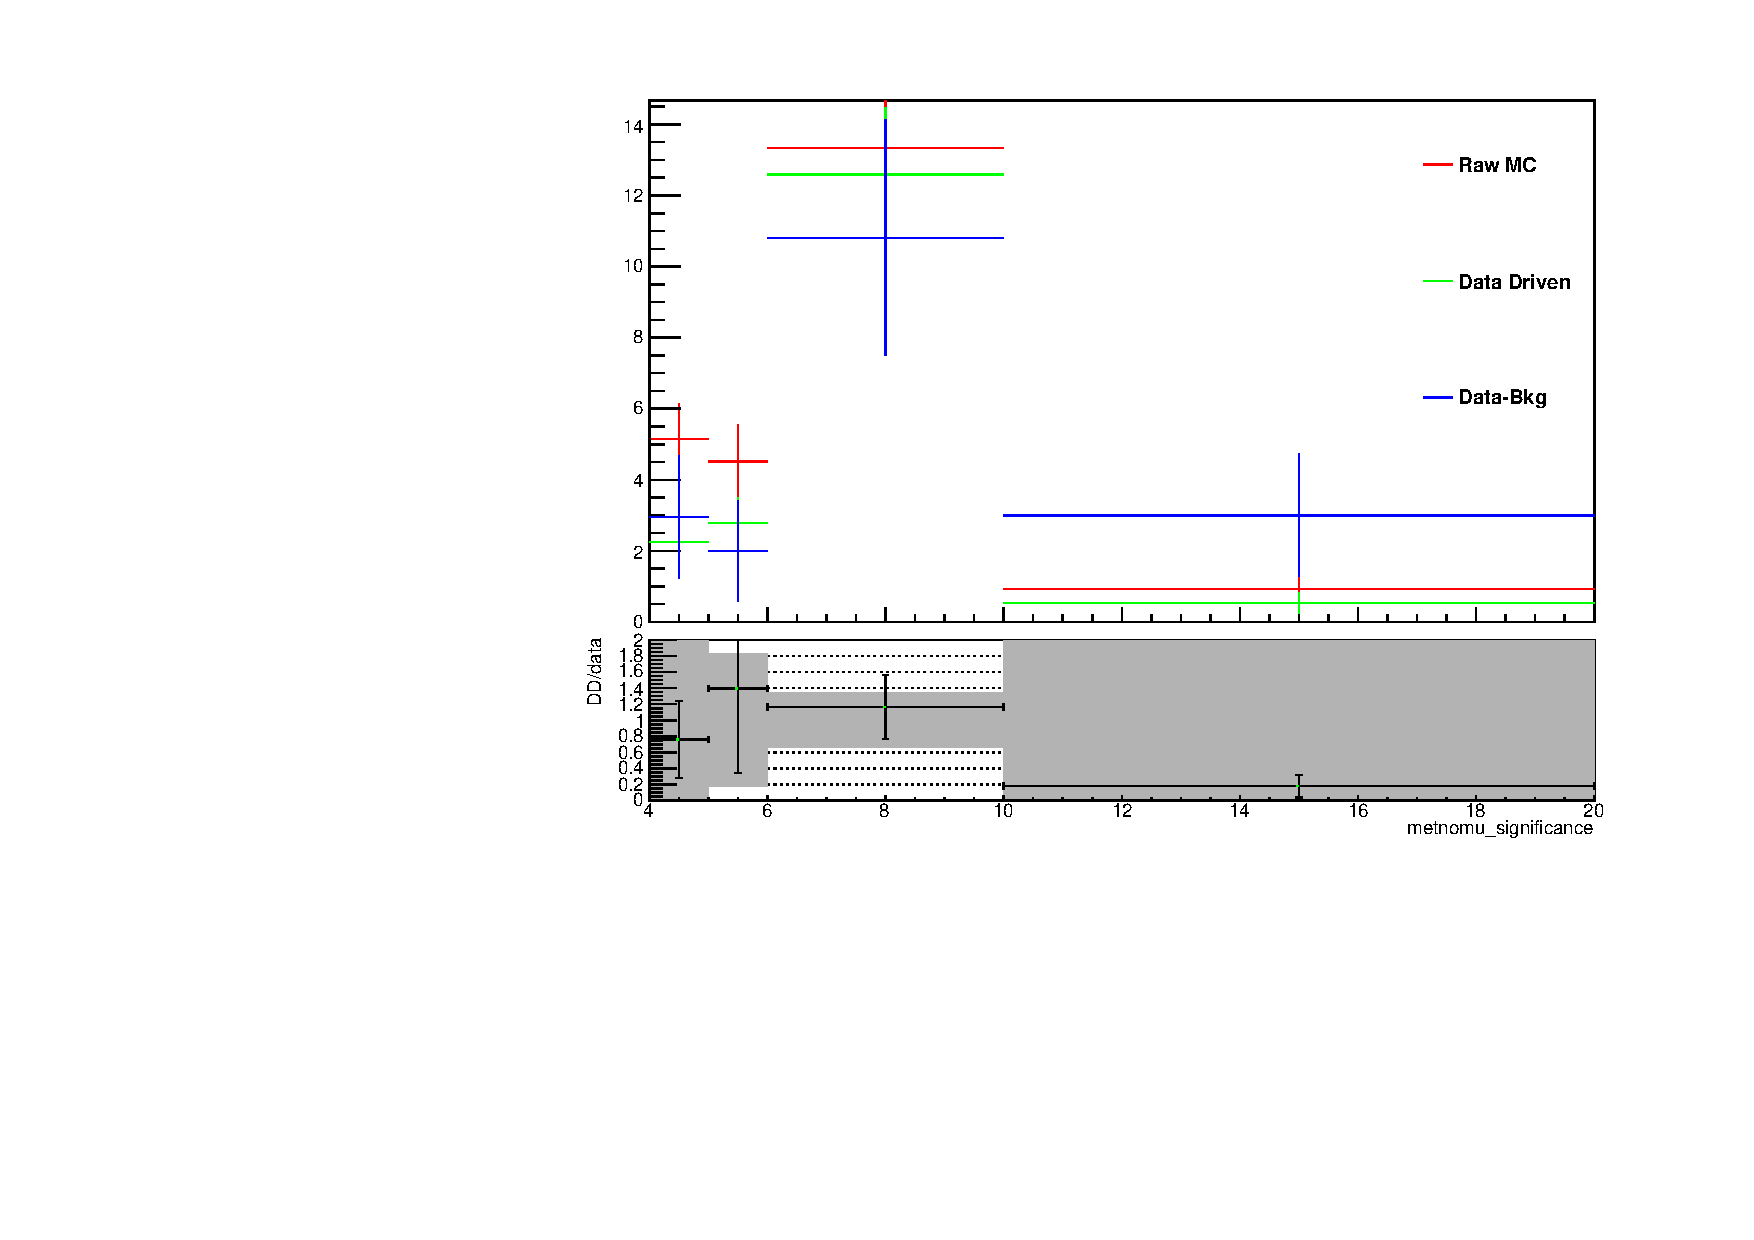
\includegraphics[width=.8\textwidth]{TalkPics/closuretests171214/closuremetnomu_significanceZJets_ll_all.pdf}
  \end{block}
\end{frame}

\begin{frame}
  \frametitle{mumu closure}
  \begin{block}{}
    \centering
    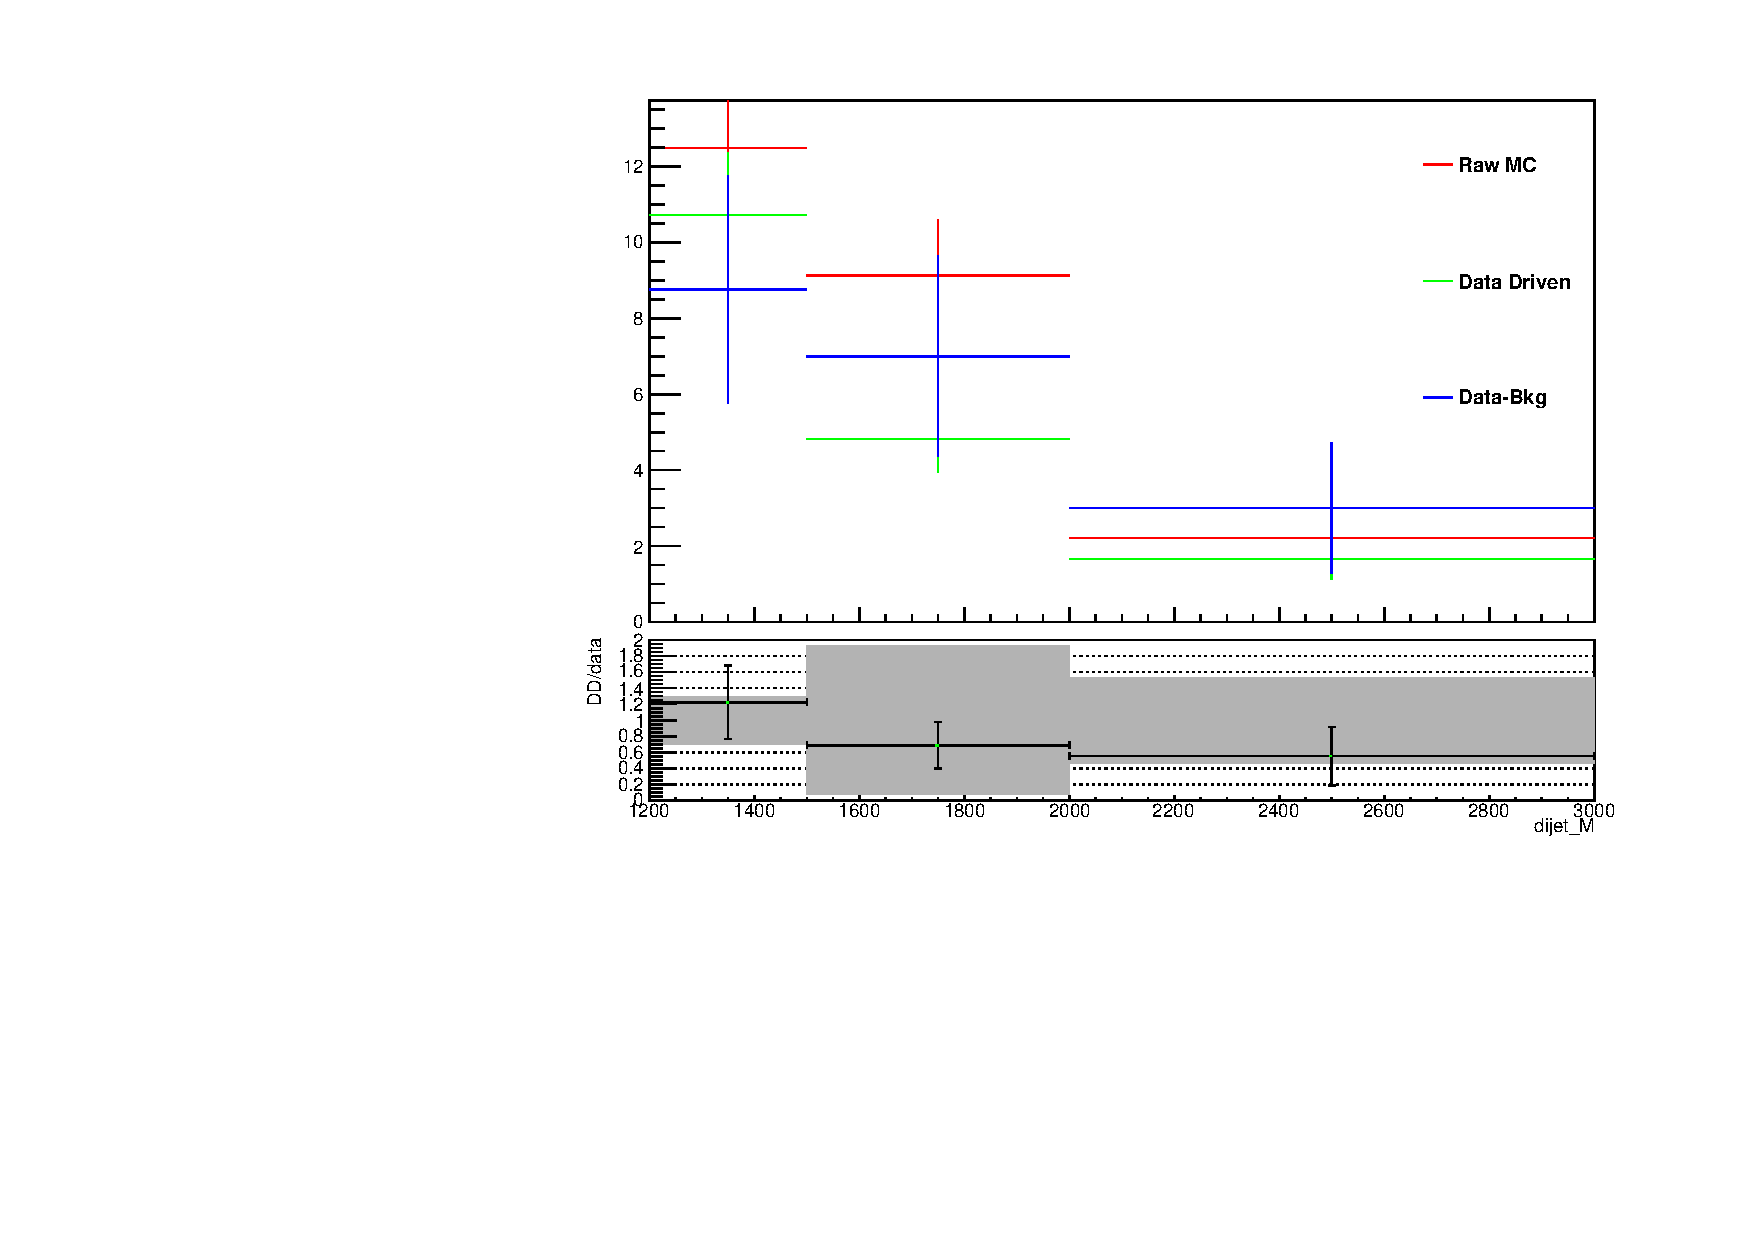
\includegraphics[width=.8\textwidth]{TalkPics/closuretests171214/closuredijet_MZJets_ll_all.pdf}
  \end{block}
\end{frame}

\begin{frame}
  \frametitle{mumu closure}
  \begin{block}{}
    \centering
    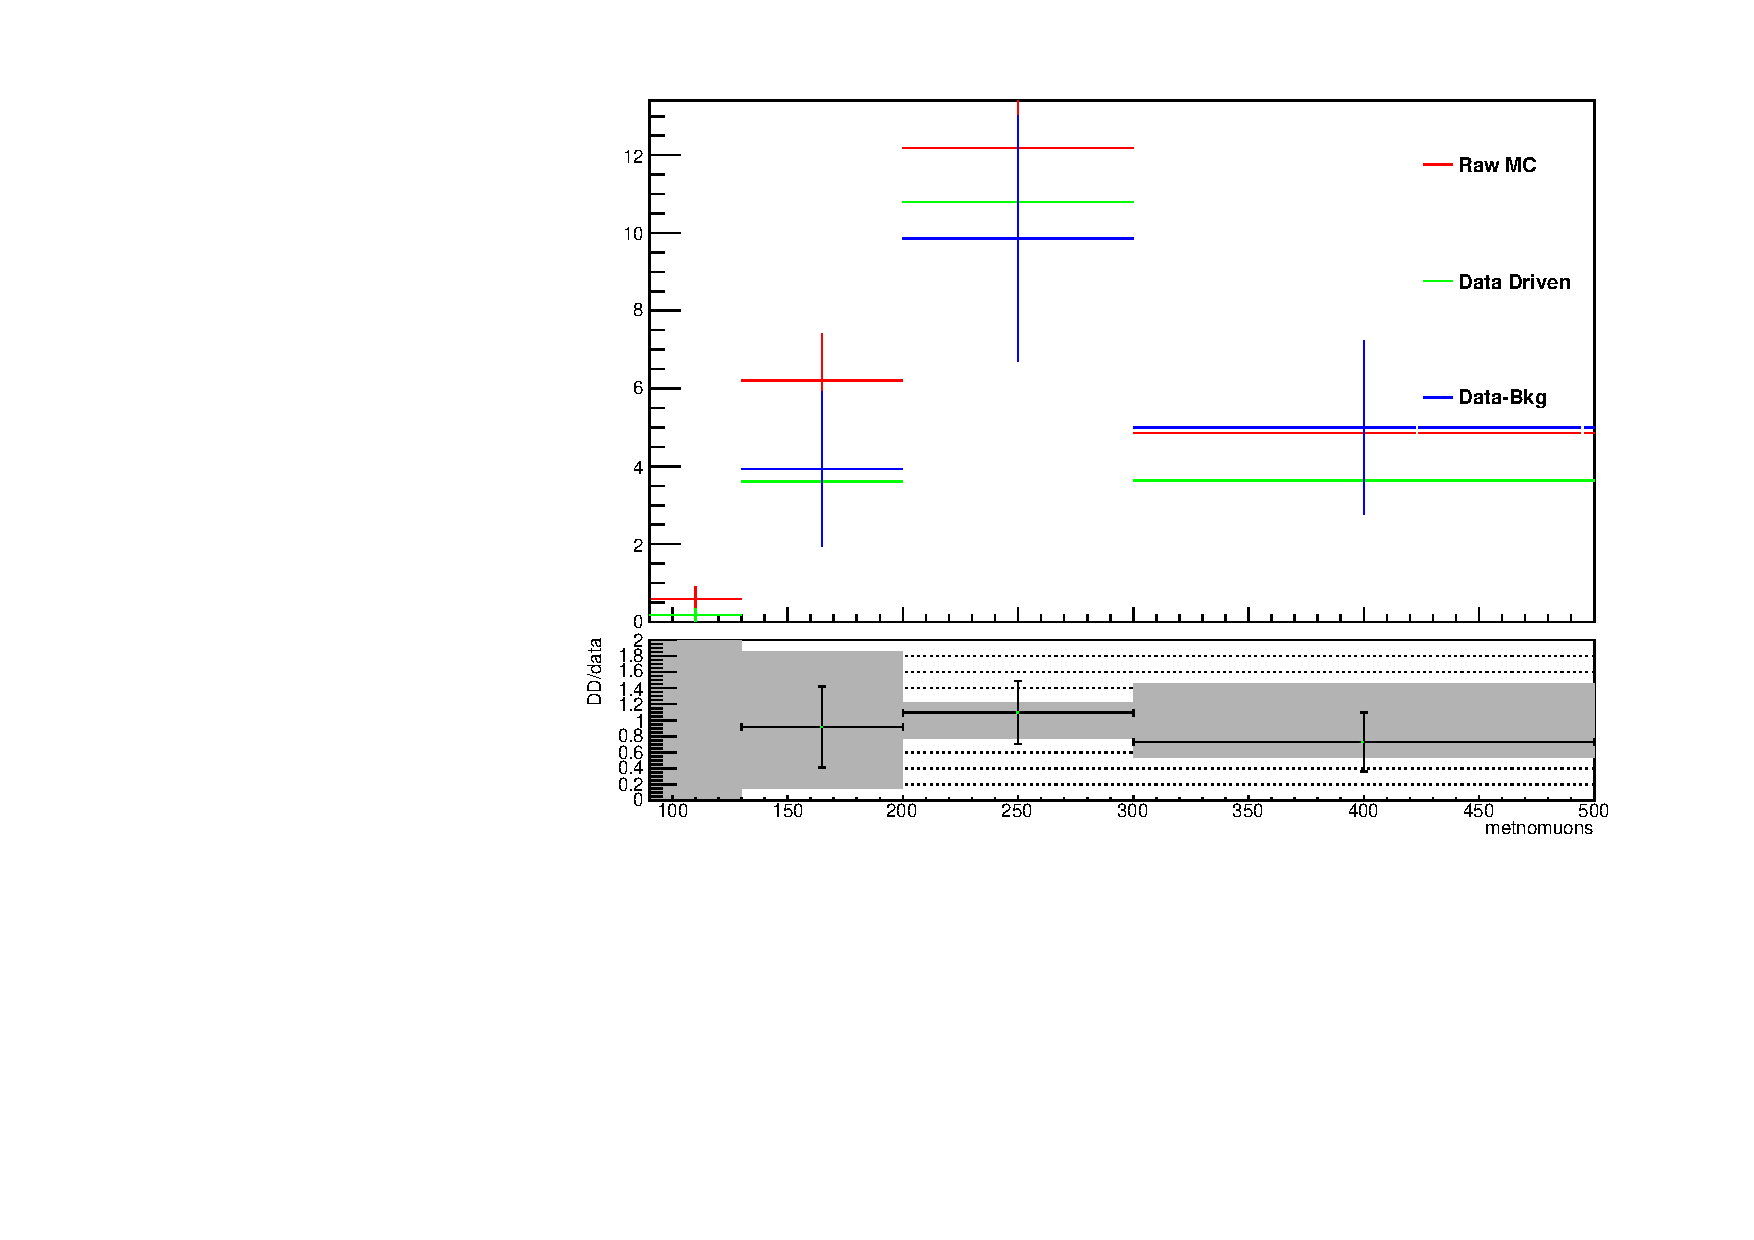
\includegraphics[width=.8\textwidth]{TalkPics/closuretests171214/closuremetnomuonsZJets_ll_all.pdf}
  \end{block}
\end{frame}


\begin{frame}
  \frametitle{Closure Test Conclusion}
  \label{lastframe}
  \begin{block}{}
    \scriptsize
    \begin{itemize}
    \item Majority of bins Data-Driven a lot closer to Data than Raw MC is
    \item Majority of Data-Driven/Data ratio points inside systematic band
    \end{itemize}
    
  \end{block}

\end{frame}

\begin{frame}
  \frametitle{Summary}
  \begin{block}{}
    \scriptsize
    \begin{itemize}
    \item Answers to preapproval conditions presented
    \item We await instructions on next steps
    \end{itemize}
  \end{block}
\end{frame}

\begin{frame}
  \frametitle{Backup}
\end{frame}

\end{fmffile}
\end{document}
